% Define important features for the document
\documentclass[12pt,oneside]{article}
\setlength{\parindent}{0pt}
\setlength{\parskip}{4pt}

% Import packages
\usepackage[margin = 1in]{geometry}
\usepackage{amsfonts, amsmath, amssymb, amsthm, calc, centernot, color, csquotes, dsfont, enumitem, environ, fancyhdr, fontawesome5, graphicx, hyperref, marvosym, mathrsfs, mathtools, tcolorbox, titlesec}
\usepackage[flushmargin,hang]{footmisc}
\tcbuselibrary{breakable}

% Define toggles
\newif\ifsolutions
\solutionstrue % Toggle for instructor version
% \solutionsfalse % Toggle for student version

% Define size and spacing of section and subsection
\titleformat{\section}
  {\normalfont\large\bfseries}
  {\thesection}{1em}{}
\titleformat{\subsection}
  {\normalfont\normalsize\bfseries}
  {\thesubsection}{1em}{}
\titlespacing*{\section}{0pt}{6pt}{6pt} % ({left}{before}{after})
\titlespacing*{\subsection}{0pt}{6pt}{6pt} % ({left}{before}{after})

% Define commands
\newcommand{\indep}{\perp\!\!\!\perp}
\newcommand{\notindep}{\mathrel{\not\!\perp\!\!\!\perp}}
\newcommand{\E}{\mathbb{E}}
\newcommand{\Var}{\text{Var}}
\newcommand{\Cov}{\text{Cov}}
\newcommand{\Corr}{\text{Corr}}
\newcommand{\SD}{\text{SD}}
\newcommand{\SE}{\text{SE}}
\newcommand{\Bias}{\text{Bias}}
\newcommand{\MSE}{\text{MSE}}
\newcommand{\Risk}{\text{Risk}}
\newcommand{\Like}{\mathcal{L}}
\newcommand{\boot}{\text{boot}}
\newcommand{\strat}{\text{strat}}
\newcommand{\supp}{\text{supp}}
\newcommand{\MLE}{\text{MLE}}
\newcommand{\MoM}{\text{MoM}}
\newcommand{\MOM}{\text{MOM}}
\newcommand{\OLS}{\text{OLS}}
\newcommand{\WLS}{\text{WLS}}
\newcommand{\LS}{\text{LS}}
\newcommand{\MAP}{\text{MAP}}
\newcommand{\MAE}{\text{MAE}}
\newcommand{\LP}{\text{LP}}
\newcommand{\HT}{\text{HT}}
\newcommand{\JS}{\text{JS}}
\newcommand{\RB}{\text{RB}}
\newcommand{\UB}{\text{UB}}
\newcommand{\DIM}{\text{DIM}}
\newcommand{\PATE}{\text{PATE}}
\newcommand{\SATE}{\text{SATE}}
\newcommand{\VIF}{\text{VIF}}
\newcommand{\GVIF}{\text{GVIF}}
\newcommand{\AIC}{\text{AIC}}
\newcommand{\BIC}{\text{BIC}}
\newcommand{\LASSO}{\text{LASSO}}
\newcommand{\PSS}{\text{PSS}}
\newcommand{\CV}{\text{CV}}
\newcommand{\logit}{\text{logit}}
\newcommand{\odds}{\text{odds}}
\newcommand{\OR}{\text{OR}}
\newcommand{\N}{\mathcal{N}}
\newcommand{\Bern}{\text{Bern}}
\newcommand{\Bin}{\text{Bin}}
\newcommand{\Beta}{\text{Beta}}
\newcommand{\Gam}{\text{Gamma}}
\newcommand{\Expo}{\text{Expo}}
\newcommand{\Pois}{\text{Pois}}
\newcommand{\Unif}{\text{Unif}}
\newcommand{\DUnif}{\text{DUnif}}
\newcommand{\Geom}{\text{Geom}}
\newcommand{\FS}{\text{FS}}
\newcommand{\NBin}{\text{NBin}}
\newcommand{\HGeom}{\text{HGeom}}
\newcommand{\Mult}{\text{Mult}}
\newcommand{\MVN}{\text{MVN}}
\newcommand{\IG}{\text{IG}}
\newcommand{\Tweedie}{\text{Tweedie}}
\newcommand{\simiid}{\overset{\text{i.i.d.}}{\sim}}
\newcommand{\simind}{\overset{\text{ind.}}{\sim}}
\newcommand{\simnull}{\overset{H_0}{\sim}}
\newcommand{\simapprox}{\overset{\cdot}{\sim}}
\newcommand{\simnullapprox}{\overset{H_0}{\simapprox}}
\newcommand{\R}{\mathbb{R}}
\newcommand{\Z}{\mathbb{Z}}
\newcommand{\Q}{\mathbb{Q}}
\newcommand{\C}{\mathbb{C}}
\newcommand{\I}{\mathbb{I}}
\newcommand{\indic}{\mathds{1}}
\newcommand{\iid}{\text{i.i.d.}}
\newcommand{\Ind}{\text{Ind}}
\newcommand{\SSq}{\text{SSq}}
\newcommand{\trace}{\text{trace}}
\newcommand{\rank}{\text{rank}}
\newcommand{\diag}{\text{diag}}
\newcommand{\adj}{\text{adj}}
\newcommand{\SSE}{\text{SSE}}
\newcommand{\SST}{\text{SST}}
\newcommand{\SSR}{\text{SSR}}
\newcommand{\GLS}{\text{GLS}}
\newcommand{\df}{\text{df}}
\newcommand{\ti}{\text{time}}
\newcommand{\outcome}{\text{outcome}}
\newcommand{\exposure}{\text{exposure}}
\newcommand{\NA}{\text{NA}}
\newcommand{\cp}{\text{cp}}
\newcommand{\tip}{\textbf{\faLightbulb}: }
\newcommand{\warning}{\textbf{\Biohazard}: }
\newcommand{\blank}[1][4cm]{\underline{\hspace{#1}}}

% Define theorem-style environment (italic body, bold header)
\newtheorem{theorem}{Theorem}
\newtheorem{lemma}{Lemma}
\newtheorem{proposition}{Proposition}
\newtheorem{corollary}{Corollary}

% Define definition-style environment (upright body, bold header)
\theoremstyle{definition}
\newtheorem{definition}{Definition}
\newtheorem{example}{Example}
\newtheorem{problem}{\faPen \ Problem}
\newtheorem{concept}{\faPen \ Concept Checker}
\newtheorem{challenge}{\faFire \ Challenge}
\newtheorem{activity}{\faDiceThree \ Activity}

% Define idea-style environment (unnumbered definition)
\newtheorem*{idea}{Idea}

% Define remark-style environment (upright body, italic header)
\theoremstyle{remark}
\newtheorem{remark}{Remark}

% Define environment for solution box
\newsavebox{\solutioncontentbox}
\NewEnviron{solutionbox}[1][Solution]{
  \sbox{\solutioncontentbox}{
    \begin{minipage}{\dimexpr\linewidth-2\fboxsep\relax}
      \BODY
    \end{minipage}
  }
  \ifsolutions
    \begin{tcolorbox}[
      title=#1,
      colback=gray!5,
      colframe=black,
      breakable
    ]
      \BODY
    \end{tcolorbox}
  \else
    \begin{tcolorbox}[
      title=#1,
      colback=white,
      colframe=black,
      breakable,
      height=\dimexpr\ht\solutioncontentbox+\dp\solutioncontentbox+1cm\relax
    ]
    \end{tcolorbox}
  \fi
}

% Begin document
\begin{document}
\pagestyle{fancy}
\fancyhead[L]{STAT 139: Introduction to Linear Models}
\fancyhead[R]{Fall 2026}
\begin{center}
\bf \Large
Section 2: Two Sample Tests and Resampling \\[0.5em]
\normalsize
STAT 139 Teaching Team
\end{center}

% Section: Introduction
\section{Introduction}

\subsection{Logistics}

Welcome! The goal of our weekly section is to review content from lecture, with emphasis on big-picture intuition, mathematical derivation, and hands-on practice.

Specifically, we aim for section to be interactive, well-paced, inclusive, and fun! Please do not hesitate to reach out if you have any questions/feedback!

\subsection{Office Hours}

$\bullet$ See Canvas for the most accurate information!

\subsection{Attendance}

$\bullet$ Please notify the Teaching Fellow (TF) if your attendance hasn't been taken!

% Section: Inference for Proportions
\section{Inference for Proportions}

\begin{idea}
Broadly, \textit{inference} can be split into two scenarios: inference for \textit{proportions}—e.g., what is the proportion of people who'll vote for a certain presidential candidate?—and inference for \textit{means}—e.g., what is the average age of people who'll vote?
\end{idea}

\subsection{Fundamentals}

\begin{center}
  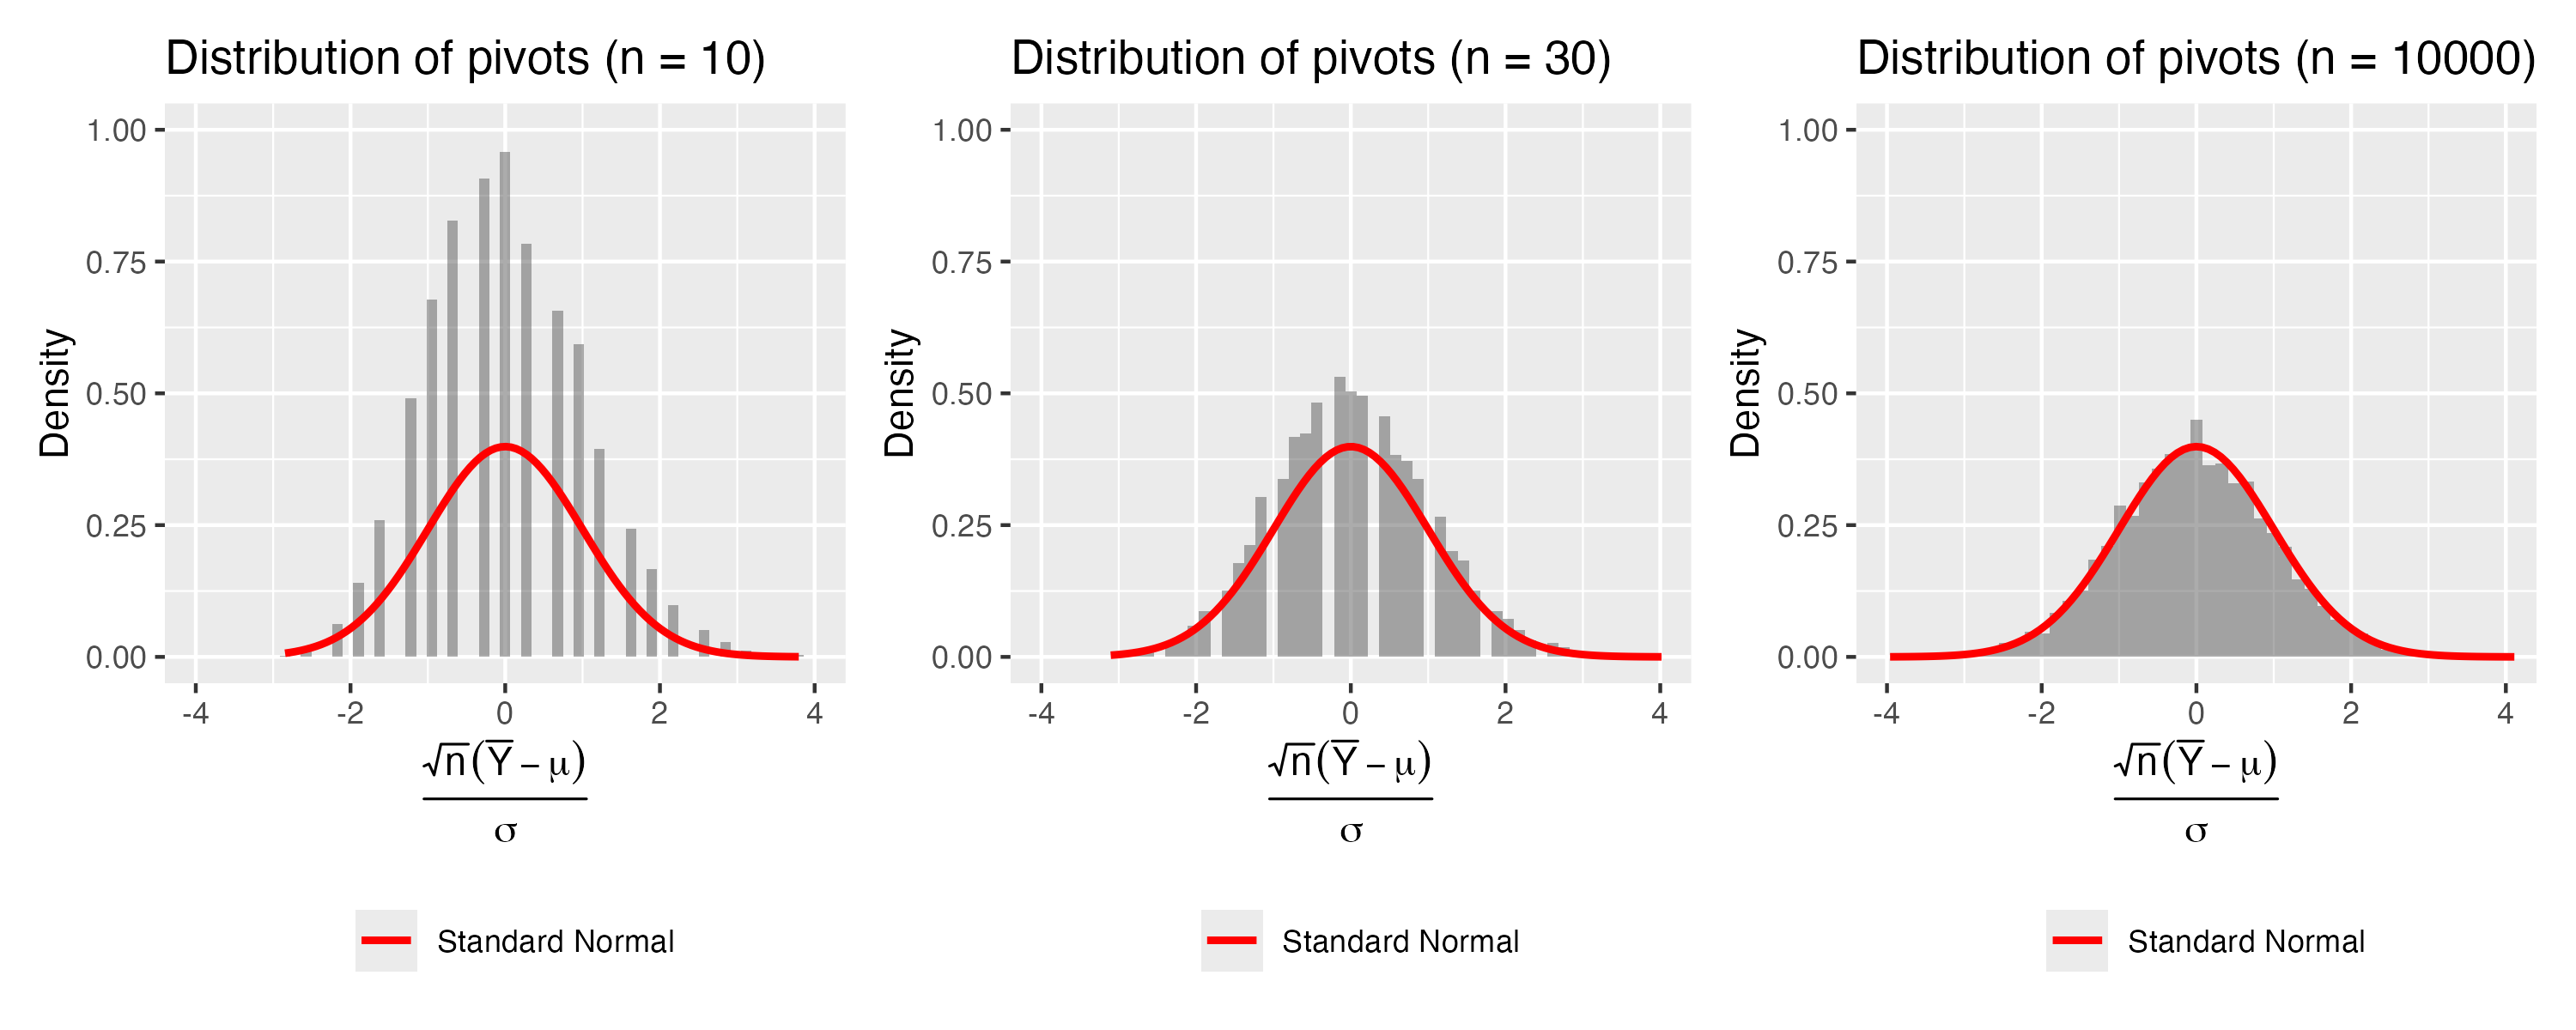
\includegraphics[width=1\textwidth]{stat139_section2_figure1.png}\\{\footnotesize FIGURE 1: $\frac{\sqrt{n}(\bar{Y} - \mu)}{\sigma}$ (in gray) converges in distribution to $\N(0, 1)$ (in red). If we \enquote{freeze} at $n = 30$, then the approximate distribution is close to the asymptotic distribution.}
\end{center}

\begin{definition}[Central Limit Theorem (CLT)]
For i.i.d. random variables $X_1, \ldots, X_n$ with finite expectation $\E[X_i] = \mu$ and finite variance $\Var[X_i] = \sigma^2$, define the \textit{sample mean} as \[\bar{X} = \frac{1}{n} \sum_{i=1}^{n} X_i.\] Then \[\sqrt{n}(\bar{X} - \mu) \xrightarrow{d} \N(0, \sigma^2).\]

$\bullet$ This implies that \[\bar{X} \simapprox \N \left( \mu, \frac{\sigma^2}{n} \right)\] for large $n$.\footnote{See Appendix~\ref{app:clt-approx}.}

$\bullet$ \Biohazard: It is incorrect to say that $\bar{X} \xrightarrow{d} \N(\mu, \frac{\sigma^2}{n})$. Why? Recall that convergence in distribution is in the limit as $n$ approaches infinity, but here, $n$ is on the right side of the equation! Thus, for each $n$, the \enquote{thing being converged to} keeps changing.
\end{definition}

\subsection{One-Sample Test for Proportions}

\begin{idea}
We begin by working with only one group. Here, the outcome for observation $i$, $X_i$, is binary, so $X_i \sim \Bern(p_i)$ for some probability $p_i$.
\end{idea}

\begin{definition}[One-sample setup]
Let $X_{1}, \ldots, X_{n} \simiid \Bern(p)$ such that $\E[X_i] = p$ and $\Var[X_i] = p(1 - p)$. Then \[\bar{X} \simapprox \N \left( p, \frac{p(1 - p)}{n} \right)\] for large $n$ by CLT.

$\bullet$ Equivalently, define $\hat{p} = \bar{X}$ as an estimator for $p$.
\end{definition}

\subsection{Two-Sample Test for Proportions}

\begin{idea}
We now extend to working with two groups of interest, whose probabilities we want to compare. Importantly, we can handle whether the two groups have different sample sizes.
\end{idea}

\begin{definition}[Two-sample setup]
Let $X_{1}, \ldots, X_{n} \simiid \Bern(p_1)$ and $Y_{1}, \ldots, Y_{m} \simiid \Bern(p_2)$, with the two samples independent. Like before, each sample has its own sample mean.

Then \[\bar{X} - \bar{Y} \simapprox \N \left( p_1 - p_2, \frac{p_1(1 - p_1)}{n} + \frac{p_2(1 - p_2)}{m} \right)\] for large $n$ and $m$ by CLT.

$\bullet$ Equivalently, define $\hat{p}_1 - \hat{p}_2 = \bar{X} - \bar{Y}$ as an estimator for $p_1 - p_2$.
\end{definition}

\begin{concept}
Why is it crucial that the two samples are independent to derive the distribution of $\bar{X} - \bar{Y}$? For the sake of simplicity, assume that $\bar{X} \sim \N \left( p_1, \frac{p_1(1 - p_1)}{n} \right)$ and $\bar{Y} \sim \N \left( p_2, \frac{p_2(1 - p_2)}{m} \right)$ are exact distributions.
\end{concept}

\begin{solutionbox}
If $\bar{X} \indep \bar{Y}$, then $\bar{X} - \bar{Y} \sim \N \left( p_1 - p_2, \frac{p_1(1 - p_1)}{n} + \frac{p_2(1 - p_2)}{m} \right)$ by shifting/scaling of independent Normals. If $\bar{X} \notindep \bar{Y}$, then this doesn't hold.
\end{solutionbox}

% Section: Inference for Means
\section{Inference for Means}

\begin{idea}
The $t$-distribution is often used in linear models, especially when we don't know the population variance $\sigma^2$ and must plug in an estimator. As expected, the $t$-distribution accounts for this extra uncertainty/variability, but as $n$ increases, it becomes more Normal.
\end{idea}

\subsection{Fundamentals}

\begin{center}
  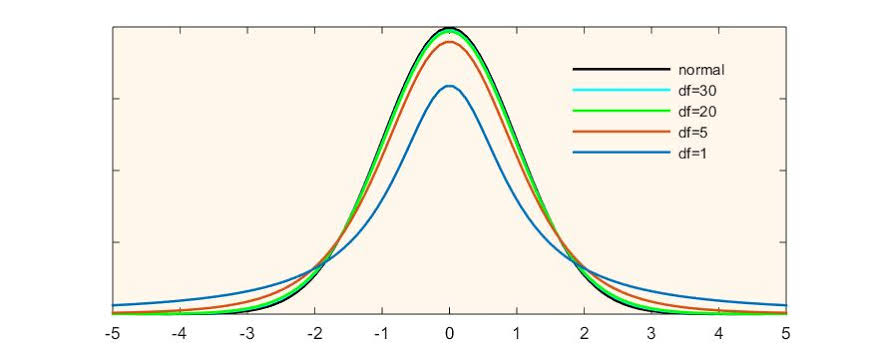
\includegraphics[width=1\textwidth]{stat139_section2_figure2.jpg}\\{\footnotesize FIGURE 2: The $t$-distribution asymptotically approaches $\N(0, 1)$ (in black).}
\end{center}

\begin{definition}[$t$-distribution]
Let $Z \sim \N(0, 1)$ and $Y \sim \chi^{2}_{\nu}$, with $Z \indep Y$. Then \[T = \frac{Z}{\sqrt{Y / \nu}} \sim t_{\nu}\]

$\bullet$ As shown by Figure 2, $T$ converges in distribution to $\N(0, 1)$ as $\nu \rightarrow \infty$.
\end{definition}

\subsection{One-Sample Tests for Means}

\begin{idea}
We begin by working with only one group. Here, the outcome for observation $i$, $X_i$, is continuous (usually, any real number), so $X_i$ can be Normal—or it can be some other distribution entirely!
\end{idea}

\begin{definition}[One-sample setup]
Let $X_{1}, \ldots, X_{n} \simiid \N(\mu, \sigma^2)$ such that $\E[X_i] = \mu$ and $\Var[X_i] = \sigma^2$. Define the \textit{sample variance}\footnote{We define the sample variance as the unbiased estimator for variance (even though other estimators exist).} as \[S^2 = \frac{1}{n - 1} \sum_{i = 1}^{n} (X_{i} - \bar{X})^2.\] Then \[\bar{X} \sim \N \left( \mu, \frac{\sigma^2}{n} \right)\] and \[\frac{n - 1}{\sigma^{2}} S^{2} \sim \chi^{2}_{n - 1}.\]
\end{definition}

\begin{concept}
Let $X_{1}, \ldots, X_{n} \simiid \N(\mu, \sigma^2)$. Show that $\bar{X} \sim \N \left( \mu, \frac{\sigma^2}{n} \right)$. Is this an approximate distribution?
\end{concept}

\begin{solutionbox}
First, $\bar{X} = \frac{1}{n} \sum_{i = 1}^{n} X_{i}$, so it is Normal as a linear combination of Normals. Thus, we need to find $\E[\bar{X}]$ and $\Var[\bar{X}]$.

\[
\begin{aligned}
\E[\bar{X}] &= \E \left[ \frac{1}{n} \sum_{i = 1}^{n} X_{i} \right] && \text{since $\bar{X} = \frac{1}{n} \sum_{i = 1}^{n} X_{i}$} \\
&= \frac{1}{n} \sum_{i = 1}^{n} \E[X_{i}] && \text{by linearity} \\
&= \frac{1}{n} \sum_{i = 1}^{n} \mu && \text{since $\E[X_{i}] = \mu$} \\
&= \mu && \text{by simplifying}
\end{aligned}
\]

\[
\begin{aligned}
\Var[\bar{X}] &= \Var \left[ \frac{1}{n} \sum_{i = 1}^{n} X_{i} \right] && \text{since $\bar{X} = \frac{1}{n} \sum_{i = 1}^{n} X_{i}$} \\
&= \frac{1}{n^2} \left( \sum_{i = 1}^{n} \Var[X_{i}] + 2 \sum_{i < j} \Cov[X_{i}, X_{j}] \right) && \text{by bilinearity} \\
&= \frac{1}{n^2} \left( \sum_{i = 1}^{n} \Var[X_{i}] \right) && \text{by independence} \\
&= \frac{1}{n^2} \left( \sum_{i = 1}^{n} \sigma^2 \right) && \text{since $\Var[X_{i}] = \sigma^2$} \\
&= \frac{\sigma^2}{n} && \text{by simplifying}
\end{aligned}
\]

Thus, $\bar{X} \sim \N \left( \mu, \frac{\sigma^2}{n} \right)$. This is an exact distribution—we do not rely on asymptotics/CLT but rather properties of the Normal!
\end{solutionbox}

\begin{definition}[One-sample $z$-test, $\sigma^2$ known]
We want to conduct the two-sided test $H_{0}: \mu = \mu_{0}$ vs. $H_{A}: \mu \neq \mu_{0}$, with $\sigma^2$ known. We use \[Z = \frac{\bar{X} - \mu_{0}}{\sigma / \sqrt{n}} \simnull \N(0, 1)\] as our \textit{test statistic} (i.e., its \textit{exact} distribution is known under $H_0$).
\end{definition}

\begin{definition}[One-sample $t$-test, $\sigma^2$ unknown]
We want to conduct the two-sided test $H_{0}: \mu = \mu_{0}$ vs. $H_{A}: \mu \neq \mu_{0}$, with $\sigma^2$ unknown. We use \[T = \frac{\bar{X} - \mu_{0}}{S / \sqrt{n}} \simnull t_{n - 1}\] as our \textit{test statistic} (i.e., its \textit{exact} distribution is known under $H_0$).
\end{definition}

\begin{concept}
For the one-sample $z$-test where $\sigma^2$ is known, why is it critical that we assume the null hypothesis? Does the distribution hold under the alternative hypothesis?
\end{concept}

\begin{solutionbox}
Even though $\mu$ is unknown at the end of the day, if we assume the null hypothesis, then we insert a known value for $\mu$ (e.g., $\mu_0 = 139$), which allows us to calculate the statistic and know its distribution. Specifically, $\frac{\bar{X} - \mu}{\sigma / \sqrt{n}} \sim \N(0, 1)$ by standardizing the distribution of $\bar{X}$ (no null hypothesis needed), but in order to actually subtract a value for $\mu$ in practice, we must use a null value (i.e., $\mu_0$). Under $H_0: \mu = \mu_0$, $\frac{\bar{X} - \mu_0}{\sigma / \sqrt{n}} \sim \N(0, 1)$, but if $\mu \neq \mu_0$, then $\frac{\bar{X} - \mu_0}{\sigma / \sqrt{n}} \sim \N \left( \frac{\mu - \mu_0}{\sigma / \sqrt{n}}, 1 \right)$.
\end{solutionbox}

\subsection{Four Setups in One-Sample Inference for Means}

\begin{idea}
If the data are Normal, we conduct \textit{finite-sample inference} using exact distributions. But even with non-Normal data, we can appeal to CLT. Thus, depending on whether the data are Normal and whether $\sigma^2$ is known, there are four scenarios. Let $z_{1 - \frac{\alpha}{2}}$ be the $1 - \frac{\alpha}{2}$ critical value of the $\N(0, 1)$ distribution and $t_{1 - \frac{\alpha}{2}, n - 1}$ be the $1 - \frac{\alpha}{2}$ critical value of the $t_{n - 1}$ distribution.\footnote{Equivalently, $z_{1 - \frac{\alpha}{2}} = Q_{\N(0, 1)}(1 - \frac{\alpha}{2})$ and $t_{1 - \frac{\alpha}{2}, n - 1} = Q_{t_{n - 1}}(1 - \frac{\alpha}{2})$, where $Q(x) = F^{-1}(x)$ is the quantile function.}
\end{idea}

\begin{center}
\renewcommand{\arraystretch}{1.5}
\begin{tabular}{p{6cm}|p{5cm}|p{5cm}}
\textbf{Data} & 
\textbf{Test Stat and Distribution under $H_0: \mu = \mu_0$} & 
\textbf{Confidence Interval for $\mu$} \\ \hline

$X_1, \ldots, X_n \simiid \N(\mu, \sigma^2)$, $\mu$ unknown, $\sigma^2$ known
& $\frac{\bar{X} - \mu_0}{\sigma / \sqrt{n}} \simnull \N(0, 1)$
& $\bar{X} \pm z_{1 - \frac{\alpha}{2}} \times \frac{\sigma}{\sqrt{n}}$ \\

\hline

$X_1, \ldots, X_n \simiid \N(\mu, \sigma^2)$, $\mu$ and $\sigma^2$ unknown
& $\frac{\bar{X} - \mu_0}{S / \sqrt{n}} \simnull t_{n - 1}$
& $\bar{X} \pm t_{1 - \frac{\alpha}{2}, n - 1} \times \frac{S}{\sqrt{n}}$ \\

\hline

$X_1, \ldots, X_n$ i.i.d., $\mu$ unknown, $\sigma^2$ known
& $\frac{\bar{X} - \mu_0}{\sigma / \sqrt{n}} \simnullapprox \N(0, 1)$ for large $n$
& $\bar{X} \pm z_{1 - \frac{\alpha}{2}} \times \frac{\sigma}{\sqrt{n}}$ \\

\hline

$X_1, \ldots, X_n$ i.i.d., $\mu$ and $\sigma^2$ unknown
& $\frac{\bar{X} - \mu_0}{S / \sqrt{n}} \simnullapprox \N(0, 1)$ for large $n$
& $\bar{X} \pm z_{1 - \frac{\alpha}{2}} \times \frac{S}{\sqrt{n}}$
\end{tabular}
\end{center}

\begin{concept}
In one-sample inference, why are there more possible scenarios for means than for proportions?
\end{concept}

\begin{solutionbox}
In one-sample inference for proportions, only $p = \E[X_i]$ is unknown (if we knew $p$, then we'd know $\Var[X_i] = p(1 - p)$). Thus, we only have one estimator: $\hat{p} = \bar{X}$. But in one-sample inference for means, both $\mu = \E[X_i]$ and $\sigma^2 = \Var[X_i]$ are unknown (and knowing only $\mu$ is not enough for $\sigma^2$). Also, the outcome being continuous does not mean that $X_i$ is Normal (whereas the outcome being binary means that $X_i$ is Bernoulli). Thus, our scenario changes depending on whether $\sigma^2$ is known or not and whether the data are Normal or not.
\end{solutionbox}

\subsection{Two-Sample Tests for Means}

\begin{idea}
We now extend to working with two groups of interest, whose means we want to compare. Importantly, we can handle whether the two groups have different sample sizes and whether they have different variances.
\end{idea}

\begin{definition}[Two-sample setup]
Let $X_{1}, \ldots, X_{n} \simiid \N(\mu_{1}, \sigma^2_{1})$ and $Y_{1}, \ldots, Y_{m} \simiid \N(\mu_{2}, \sigma^2_{2})$, with the two samples independent. Like before, each sample has its own sample mean and sample variance.
\end{definition}

\begin{definition}[Two-sample $t$-test, unpooled]
We want to conduct the two-sided test $H_{0}: \mu_1 = \mu_2$ vs. $H_{A}: \mu_1 \neq \mu_2$, with $\sigma^2_1$ and $\sigma^2_2$ unknown. We \textit{don't} assume that $\sigma^2_1 = \sigma^2_2$. We use \[T = \frac{\bar{X} - \bar{Y}}{\sqrt{\frac{S^2_1}{n} + \frac{S^2_2}{m}}} \simnullapprox t_{k}\] as our \textit{test statistic} (i.e., its \textit{approximate} distribution is known under $H_0$), where $S^2_i$ is the sample variance for group $i$ and $k$ is the degrees of freedom.

$\bullet$ With computational tools like \texttt{R}, $k$ is calculated using the \textit{Satterthwaite approximation}.
\end{definition}

\begin{definition}[Two-sample $t$-test, pooled]
We want to conduct the two-sided test $H_{0}: \mu_1 = \mu_2$ vs. $H_{A}: \mu_1 \neq \mu_2$, with $\sigma^2_1$ and $\sigma^2_2$ unknown. We \textit{do} assume that $\sigma^2_1 = \sigma^2_2$. We use \[T = \frac{\bar{X} - \bar{Y}}{S_p \sqrt{\frac{1}{n} + \frac{1}{m}}} \simnull t_{n + m - 2}\] as our \textit{test statistic} (i.e., its \textit{exact} distribution is known under $H_0$), where \[S_p = \sqrt{\frac{(n - 1) S^2_1 + (m - 1) S^2_2}{n + m - 2}}\] is the pooled sample standard deviation.
\end{definition}

% Section: Bootstrapping
\section{Bootstrapping}

\begin{idea}
The \textit{bootstrap} is a powerful idea based on \textit{resampling} our data. Through this, we can conduct inference to learn more about our estimator (specifically, by approximating its \textit{standard error}). Specifically, the bootstrap is an alternative to using a theoretical sampling distribution when standard errors or confidence intervals are difficult to derive analytically.
\end{idea}

\subsection{Fundamentals}

\begin{definition}[Bootstrap]
Let $\vec{y} = (y_1, \ldots, y_n)$ be the \textit{observed} dataset, assumed to be i.i.d. from some unknown CDF $F$. We create a synthetic dataset \[\vec{Y}^* = (Y^*_1, \ldots, Y^*_n)\] by performing a simple random sample (SRS) with replacement from $\vec{y}$. We call $\vec{Y}^*$ a \textit{bootstrap sample}.

$\bullet$ Equivalently, \[Y^*_j \simiid \hat{F}\] for all $j \in \{1, \ldots, n\}$, where $\hat{F}$ is the empirical CDF of $\vec{y}$—i.e., \[\hat{F}(y) = \frac{1}{n} \sum_{j = 1}^{n} \indic\{y_j \leq y\}.\]

$\bullet$ \textit{Bootstrapping} involves generating $B$ independent bootstrap samples, each of size $n$, and using those bootstrap samples for inferential tasks.
\end{definition}

\begin{concept}
Though the observed dataset $\vec{y}$ is crystallized, why is the bootstrap sample $\vec{Y}^*$ random?
\end{concept}

\begin{solutionbox}
There is randomness in which observations we resample. E.g., if $\vec{y} = (110, 111, 139)$, then $Y^*_1$ is random since it could be $110$, $111$, or $139$ (each with $p = \frac{1}{3}$).
\end{solutionbox}

\begin{definition}[Real world]
$F$ generates $\vec{Y}$, which generates $\hat{\theta}$. We regard $\hat{\theta}$ as an \textit{estimate} for $\theta$.
\end{definition}

\begin{definition}[Bootstrap world]
$\hat{F}$ generates $\vec{Y}^*$, which generates $\hat{\theta}^*$. We regard $\hat{\theta}^*_1, \ldots, \hat{\theta}^*_B$ as \textit{estimates} for $\hat{\theta}$, where $\hat{\theta}^*_b$ is a statistic calculated from the $b$th bootstrap sample $\vec{Y}^*_b$. We define the following bootstrap-world quantities, where we use the \textit{bootstrap expectation}\footnote{See Appendix~\ref{app:boot-exp}.} (i.e., w.r.t. the randomness from sampling with replacement from $\hat{F}$, conditional on $\vec{y}$):

\[\SE_{\boot}[\hat{\theta}^*] = \sqrt{\E_{\boot}[(\hat{\theta}^* - \E_{\boot}[\hat{\theta}^*])^2]}\]

and

\[F_{\boot}(\theta) = P_{\boot}(\hat{\theta}^* \leq \theta).\]
\end{definition}

\begin{definition}[Connection between worlds]
Since $\hat{F}(y) \xrightarrow{p} F(y)$ by LLN, $\hat{F}$ is likely to approximate $F$ well if $n$ is sufficiently large.
\end{definition}

\begin{definition}[Computational cost of bootstrap]
Since each of the $n$ observations in a bootstrap sample can be any of the $n$ observed values, there are $n^n$ possible bootstrap samples, which can be very computationally expensive.\footnote{E.g., for $n = 30$, $30^{30} \approx 2 \times 10^{44}$, which is larger than the number of stars in the observable universe!} 

$\bullet$ Thus, in practice, we use \textit{Monte Carlo estimation}, where we randomly generate only $B < n^n$ bootstrap samples and use these to estimate the desired bootstrap quantity.
\end{definition}

\begin{definition}[Monte Carlo estimation]
\textit{Monte Carlo estimation} works since the bootstrap replications $\hat{\theta}^*_1, \ldots, \hat{\theta}^*_B$ are i.i.d. draws from the bootstrap world, so each estimator converges in probability to its respective bootstrap-world quantity as $B \rightarrow \infty$ by LLN. We use the bootstrap replications to calculate the following estimators:

\[\hat{\E}_{\boot}[\hat{\theta}^*] = \bar{\theta}^* = \frac{1}{B} \sum_{b = 1}^{B} \hat{\theta}^*_b \xrightarrow{p} \E_{\boot}[\hat{\theta}^*],\]

\[\widehat{\SE}_{\boot}[\hat{\theta}^*] = \sqrt{\frac{1}{B - 1} \sum_{b = 1}^{B} (\hat{\theta}^*_b - \bar{\theta}^*)^2} \xrightarrow{p} \SE_{\boot}[\hat{\theta}^*],\] and

\[\hat{F}_{\boot}(\theta) = \frac{1}{B} \sum_{b = 1}^{B} \indic\{\hat{\theta}^*_b \leq \theta\} \xrightarrow{p} F_{\boot}(\theta).\]
\end{definition}

\begin{example}[Standard error]
We want \[\SE[\hat{\theta}] = \sqrt{\E[(\hat{\theta} - \E[\hat{\theta}])^2]}.\] We can approximate this with \[\SE_{\boot}[\hat{\theta}^*] = \sqrt{\E_{\boot}[(\hat{\theta}^* - \E_{\boot}[\hat{\theta}^*])^2]}.\] But this is often computationally expensive, so in practice, we estimate it with \[\widehat{\SE}_{\boot}[\hat{\theta}^*] = \sqrt{\frac{1}{B - 1} \sum_{b = 1}^{B} (\hat{\theta}^*_b - \bar{\theta}^*)^2}.\] Crucially, there are two different sources of error:

$\bullet$ The difference between $\SE_{\boot}[\hat{\theta}^*]$ and $\SE[\hat{\theta}]$ is caused by the use of $\hat{F}$ over $F$. This error falls as $n$ increases (for statistics where the bootstrap is consistent).

$\bullet$ The difference between $\widehat{\SE}_{\boot}[\hat{\theta}^*]$ and $\SE_{\boot}[\hat{\theta}^*]$ is caused by the use of Monte Carlo simulation. This error falls as $B$ increases, which is under our control.
\end{example}

\subsection{Bootstrap Confidence Intervals}

\begin{definition}[Setup]
Let $\theta$ be the estimand and $\hat{\theta}$ be an estimator for $\theta$. Suppose that we want to use the bootstrap to get an approximate $95\%$ confidence interval.\footnote{We choose $\alpha = 0.05$ to simplify notation, but this can be generalized to any $\alpha$.}
\end{definition}

\begin{definition}[Normal interval with bootstrap standard error]
\[\hat{\theta} \pm 1.96 \times \widehat{\SE}_{\boot}[\hat{\theta}^*].\]

$\bullet$ For some intuition, this is analogous to the confidence interval $\hat{\theta} \pm 1.96 \times \widehat{\SE}[\hat{\theta}]$ but uses the bootstrap estimate of the standard error.
\end{definition}

\begin{definition}[Percentile method]
\[\left[ \hat{\theta}^*_{(\lceil 0.025B \rceil)}, \hat{\theta}^*_{(\lceil 0.975B \rceil)} \right].\]

$\bullet$ For some intuition, this is analogous to how Bayesian credible intervals are estimated by simulation.
\end{definition}

% Section: Permutation Tests
\section{Permutation Tests}

\begin{idea}
Resampling can be extended to \textit{hypothesis tests} to compare data from two groups of interest. Like with the bootstrap, we do not assume a particular parametric distribution. Specifically, the permutation test is an alternative to the $t$-test when Normality looks suspicious.
\end{idea}

\begin{definition}[Permutation test]
Let $X_1, \ldots, X_n \simiid F_X$ for group $0$ and $Y_1, \ldots, Y_m \simiid F_Y$ for group $1$, with the two samples independent. We can use a \textit{permutation test} for the hypotheses $H_0: F_X = F_Y$ vs. $H_A: F_X \neq F_Y$ (i.e., whether or not the distribution of outcomes is related to group status).
\end{definition}

\begin{definition}[Computational cost of permutation test]
There are $\binom{n + m}{n}$ ways to break the observations into a group of size $n$ and another group of size $m$, so there are $\binom{n + m}{n}$ possible permutations, which can be very computationally expensive.

$\bullet$ Thus, in practice, we use \textit{Monte Carlo estimation}, where we randomly generate only $B < \binom{n + m}{n}$ permutations and use these to conduct our test.
\end{definition}

\begin{definition}[Monte Carlo estimation]
Let $T$ be a test statistic, chosen such that large values of $T$ are evidence against $H_0$ (e.g., $T = |\bar{X} - \bar{Y}|$). Compute $t_0$, the observed value of $T$. Generate $B$ random permutations of the data, each an SRS without replacement of $X_1, \ldots, X_n, Y_1, \ldots, Y_m$ to scramble the groups under $H_0$. For each permutation, compute the test statistic—call these $t_1, \ldots, t_B$. The $p$-value is \[P(T \geq t_0) \approx \frac{1}{B} \sum_{b = 1}^{B} \indic\{t_b \geq t_0\}.\]
\end{definition}

\begin{example}[Permutation test]
Suppose we observe $x_1 = 1$ and $x_2 = 2$ for group 0 and $y_1 = 101$ and $y_2 = 102$ for group 1, where $n = m = 2$.

$\bullet$ Intuitively, it seems like the two groups come from different data-generating processes since they differ so much in magnitude—and for $T = |\bar{X} - \bar{Y}|$, $t_0 = 100$.

$\bullet$ Under the null hypothesis that the distribution of outcomes is \textit{not} related to group status (i.e., $H_0: F_X = F_Y$), then it shouldn't matter whether we shuffle the values.

$\bullet$ E.g., for permutation 1, swap $x_1$ and $y_1$ such that $X_1^* = 101$, $X_2^* = 2$, $Y_1^* = 1$, and $Y_2^* = 102$. Here, $t_1 = 0$.

$\bullet$ We repeat this process $B$ times such that we have a distribution of $T$ under $H_0$—we compare our observed $t_0$ to this null distribution.
\end{example}

% Section: Practice Problems
\section{Practice Problems}

\begin{problem}
A company has been accused of gender discrimination, allegedly tending to pay higher salaries to men than to women. Suppose that $X_1, \ldots, X_n$ are i.i.d. draws from a theoretical distribution of salaries for men at the company and $Y_1, \ldots, Y_m$ are i.i.d. draws from a theoretical distribution of salaries for women at the same company. The salaries $X_1, \ldots, X_n, Y_1, \ldots, Y_m$ are independent but not necessarily i.i.d. Let $T = \bar{X}_n - \bar{Y}_m$. Intuitively, we would like to know whether $T$ has such a large positive value it would be implausible to observe that value (or an even larger value) if the two theoretical distributions were equal. However, $n$ and $m$ are small. The CLT is not applicable with such small sample sizes, so it is not reasonable to assume $\bar{X}_n$ and $\bar{Y}_m$ are approximately Normal.\footnote{Inspired by Problem 6 in \enquote{Stat 111 Final Exam, Spring 2025} by Joseph K. Blitzstein and Neil Shephard.}

(a) Explain how we can use a permutation test to answer our scientific question of interest.

(b) Suppose that $n = m = 2$ and the data are $X_1 = 8, X_2 = 4, Y_1 = 6, Y_2 = 2$, measured in tens of thousands of dollars. Find the $p$-value for the permutation test.
\end{problem}

\begin{solutionbox}
(a) We are interested in finding a one-sided $p$-value (this corresponds with the given test statistic—$T = \bar{X}_n - \bar{Y}_m$—and scientific question of interest—whether men are paid higher than women at this company). Let $\alpha$ be the (pre-determined) value for the nominal size of this test. First, we can compute $t_0$, the observed value of $T$ from the data at hand. Then, we can generate replications $t_1, \ldots, t_B$ of the test statistic through resampling, where $B$ is a large number (e.g., $B = 10^5$). We obtain the $b$th replication as follows:

$\bullet$ Randomly permute which salaries are in the men's group and which are in the women's group by choosing a completely random set of $n$ salaries and assigning them to the men's group (and then assigning the remaining $m$ salaries to the women's group).

$\bullet$ Let $t_b$ be the new difference in sample means between the salaries in the men's group and the salaries in the women's group for the $b$th replication.

We can compare $t_0$ with the replications (which are made under the null hypothesis). The (approximate) $p$-value is the proportion of replications that are at least as extreme as the observed value—i.e., $P(T \geq t_0) \approx \frac{1}{B} \sum_{b = 1}^{B} \indic\{t_b \geq t_0\}$. We reject $H_0$ if $P(T \geq t_0) < \alpha$.

(b) Now, if the data are $X_1 = 8, X_2 = 4, Y_1 = 6, Y_2 = 2$ with $n = m = 2$, then we can follow the procedure above to find the exact $p$-value (no Monte Carlo estimation needed). First, $t_0 = \frac{1}{2}(8 + 4) - \frac{1}{2}(6 + 2) = 2$. Next, notice that if we choose the $n = 2$ salaries in the men's group, then it is deterministic which salaries are in the women's group. There are $\binom{4}{2} = 6$ possible combinations of salaries in the men's group (where order doesn't matter since $\{8, 4\}$ and $\{4, 8\}$ both produce $\bar{X}_n = 6$ and, deterministically, $\bar{Y}_m = 4$ for $T = 2$): $\{8, 4\}$, $\{8, 6\}$, $\{8, 2\}$, $\{4, 6\}$, $\{4, 2\}$, $\{6, 2\}$. Corresponding to that order, the replications $t_1, \ldots, t_6$ of $T = \bar{X}_n - \bar{Y}_m$ would be $2$, $4$, $0$, $0$, $-4$, $-2$. Since $P(T \geq t_0) = \frac{1}{B} \sum_{b = 1}^{B} \indic\{t_b \geq t_0\}$ (i.e., the proportion of these $6$ cases where the difference in sample means is at least as large as $t_0 = 2$), the $p$-value is $P(T \geq t_0) = \frac{1}{3}$. 
\end{solutionbox}

% Appendix
\appendix
\section{Proofs}

\subsection{CLT Approximation for the Sample Mean}
\label{app:clt-approx}

\begin{proof}
Suppose that we have i.i.d. random variables $X_1, \ldots, X_n$ with finite expectation $\E[X_i] = \mu$ and finite variance $\Var[X_i] = \sigma^2$. We want to show that $\bar{X} \simapprox \N(\mu, \frac{\sigma^2}{n})$ for large $n$.

Freeze at a sufficiently large $n$ such that $\sqrt{n}(\bar{X} - \mu) \simapprox \N(0, \sigma^2)$ by CLT and definition of convergence in distribution. 

\[
\begin{aligned}
\sqrt{n}(\bar{X} - \mu) \simapprox \N(0, \sigma^2) &\implies \bar{X} - \mu \simapprox \N \left( 0, \frac{\sigma^2}{n} \right) && \text{by scaling} \\
&\implies \bar{X} \simapprox \N \left( \mu, \frac{\sigma^2}{n} \right) && \text{by shifting}
\end{aligned}
\]

Thus, $\bar{X} \simapprox \N(\mu, \frac{\sigma^2}{n})$ for large $n$.
\end{proof}

\subsection{Bootstrap Expectation}
\label{app:boot-exp}

\begin{proof}
Suppose that we generate one bootstrap sample $\vec{Y}^* = (Y^*_1, \ldots, Y^*_n)$. We want to show that the bootstrap expectation of an arbitrary point in the bootstrap sample is the observed sample mean (i.e., $\E_{\boot}[Y^*_j] = \bar{y}$ for all $j \in \{1, \ldots, n\}$).

First, $Y^*_j$, an arbitrary resampled point, is a random variable that can crystallize into any number within $\{y_1, \ldots, y_n\}$. Let $I_j$ be the sample ID of the $j$th unit resampled such that $Y^*_j = y_{I_j}$. Notice that $I_j \simiid \DUnif(1, n)$ by SRS with replacement.

\[
\begin{aligned}
\E_{\boot}[Y^*_j] &= \E_{\boot}[y_{I_j}] && \text{by substituting} \\
&= \sum_{k = 1}^{n} y_k P(I_j = k) && \text{by LOTUS} \\
&= \sum_{k = 1}^{n} y_k \frac{1}{n} && \text{by Discrete Uniform} \\
&= \frac{1}{n} \sum_{k = 1}^{n} y_k && \text{by simplifying} \\
&= \bar{y} && \text{by definition}
\end{aligned}
\]

Thus, $\E_{\boot}[Y^*_j] = \bar{y}$ for all $j \in \{1, \ldots, n\}$.
\end{proof}

\end{document}